\documentclass[a4paper,12pt]{article}
\usepackage{amsmath,amsthm,amsfonts,amssymb,amscd,amstext,vmargin,graphics,graphicx,tabularx,multicol} 
\usepackage[francais]{babel}
\usepackage[utf8]{inputenc}  
\usepackage[T1]{fontenc} 
\usepackage{pstricks-add,tikz,tkz-tab,variations}
\usepackage[autolanguage,np]{numprint} 

\setmarginsrb{2cm}{1cm}{2cm}{0.5cm}{0cm}{0cm}{0cm}{0cm} %Gauche, haut, droite, haut
\newcounter{numexo}
\newcommand{\exo}[1]{\stepcounter{numexo}\noindent{\bf Exercice~\thenumexo} : \marginpar{\hfill /#1}}
\reversemarginpar


\newcounter{enumtabi}
\newcounter{enumtaba}
\newcommand{\q}{\textbf{\stepcounter{enumtabi} \theenumtabi)}  }
\newcommand{\qa}{\textbf{\stepcounter{enumtaba} (\alph{enumtaba})} }
\newcommand{\initq}{\setcounter{enumtabi}{0}}
\newcommand{\initqa}{\setcounter{enumtaba}{0}}

\newcommand{\be}{\begin{enumerate}}
\newcommand{\ee}{\end{enumerate}}
\newcommand{\bi}{\begin{itemize}}
\newcommand{\ei}{\end{itemize}}
\newcommand{\bp}{\begin{pspicture*}}
\newcommand{\ep}{\end{pspicture*}}
\newcommand{\bt}{\begin{tabular}}
\newcommand{\et}{\end{tabular}}
\renewcommand{\tabularxcolumn}[1]{>{\centering}m{#1}} %(colonne m{} centrée, au lieu de p par défault) 
\newcommand{\tnl}{\tabularnewline}

\newcommand{\bmul}[1]{\begin{multicols}{#1}}
\newcommand{\emul}{\end{multicols}}

\newcommand{\trait}{\noindent \rule{\linewidth}{0.2mm}}
\newcommand{\hs}[1]{\hspace{#1}}
\newcommand{\vs}[1]{\vspace{#1}}

\newcommand{\N}{\mathbb{N}}
\newcommand{\Z}{\mathbb{Z}}
\newcommand{\R}{\mathbb{R}}
\newcommand{\C}{\mathbb{C}}
\newcommand{\Dcal}{\mathcal{D}}
\newcommand{\Ccal}{\mathcal{C}}
\newcommand{\mc}{\mathcal}

\newcommand{\vect}[1]{\overrightarrow{#1}}
\newcommand{\ds}{\displaystyle}
\newcommand{\eq}{\quad \Leftrightarrow \quad}
\newcommand{\vecti}{\vec{\imath}}
\newcommand{\vectj}{\vec{\jmath}}
\newcommand{\Oij}{(O;\vec{\imath}, \vec{\jmath})}
\newcommand{\OIJ}{(O;I,J)}


\newcommand{\reponse}[1][1]{%
\multido{}{#1}{\makebox[\linewidth]{\rule[0pt]{0pt}{20pt}\dotfill}
}}

\newcommand{\titre}[5] 
% #1: titre #2: haut gauche #3: bas gauche #4: haut droite #5: bas droite
{
\noindent #2 \hfill #4 \\
#3 \hfill #5

\vspace{-1.6cm}

\begin{center}\rule{6cm}{0.5mm}\end{center}
\vspace{0.2cm}
\begin{center}{\large{\textbf{#1}}}\end{center}
\begin{center}\rule{6cm}{0.5mm}\end{center}
}



\begin{document}
\pagestyle{empty}
\titre{Contrôle 2 : Fonctions affines }{Nom :}{Prénom :}{\textbf{2nd 8}}{Date:}



\exo{5.5} Les fonctions suivantes sont-elles affines ? Si oui ,donner leurs coefficients directeurs et leurs ordonnées à l'origine.\\

\initqa \qa $f(x)=-9x+6$ \qa $g(x)=3x^2+5$ \qa $h(x)=-2(4-3x)$\\

 \qa $j(x)=\dfrac{10}{3x}$ \qa $f(x)=\dfrac{x-2}{9}$\\

\vspace*{0.5cm}

\exo{4.5}On munit le plan d’un repère orthogonal.\\
Sur le graphique ci-contre, on a représenté deux fonctions $f$ et $g$ sur l'intervalle [-10;14].\\
On note $D_f$  et $D_g$ les droites qui représentent respectivement les fonctions affines $f$ et $g$.\\
\includegraphics[scale=1.5]{lecturegraphique.eps} \\

 \initq \q Quelle est l'image de -2 par la fonction $f$ ?\\

\q Quelle est l'image de 8 par la fonction $g$ ?\\

\q Déterminer $f(10)$?\\

\q Lire le ou les antécédent(s) de 8 par la fonction $f$ ??\\

\q Lire le ou les antécédent(s) de 2  par la fonction $g$ ?\\

\q Quelle est l'abscisse du point de $C_f$ d'ordonnée 5 ?\\

\q Quel est l'ensemble des solutions de l'équation $g(x)=-4$ ?\\

\q Quel est l'ensemble des solutions de l'équation $f(x)>0$ ?\\


\newpage
\vspace*{0.5cm}

\exo{6} Soient $f$ et $g$ deux fonctions affines définies par $f(x)=-3x+20$ et  $g(x)=\dfrac{5-3x}{10}$.\\

 \initq \q Calculer l'image de -3 par la fonction $f$ .\\

\q Calculer l'image de 0 par la fonction $g$ .\\

\q  Calculer $f\left(\dfrac{4}{3}\right)$.\\

\q Déterminer les antécédents éventuels de 18,5 par f .\\

\q Quelle est l'abscisse du point de $C_f$ d'ordonnée 0 ?\\

\vspace*{0.5cm}


\exo{4} Pour les trois droites représentées ci-dessous, déterminer
leurs coefficients directeurs, leurs ordonnées à l'origine puis les expressions des fonctions affines correspondant aux droites.\\


\includegraphics[scale=1.8]{representation2.eps} \\
\vspace*{0.5cm}


\exo{} \textbf{BONUS} \\
\textbf{Reprenons l'exercice 2.} D'abord graphiquement puis par le calcul, déterminer l'ensemble des solutions de l'équation $f(x)=g(x)$?\\

\end{document}
